\documentclass{article}

\usepackage[utf8]{inputenc}
\usepackage[T1]{fontenc}
\usepackage[frenchb]{babel}

\usepackage{a4wide}

\usepackage{amsmath}
\usepackage{amssymb}
\usepackage{amsthm}

\usepackage{hyperref}

\usepackage{graphicx}

\title{Heuristic Optimization: implementation exercise 2}
\author{Samuel Buchet: 000447808}
\date{May 2017}

\begin{document}

\maketitle

\section{Introduction}

Two stochastic local search algorithms are implemented for this second implementation exercise.
The first one is a Simulated Annealing (SA), which belongs to the class of simple stochastic algorithms.
The second one is a Greedy Randomised Adaptive Search Procedures (GRASP), which is a hybrid stochastic algorithm.

\section{Metaheuristics}

\subsection{Simulated annealing}

\subsubsection{Principle}

The first metaheuristic implemented is the simulated annealing algorithm.
This algorithm is made on the basis of a local search.
The neighbourhood used is the transpose one because it is the smallest one.
Thanks to this small neighbourhood, it is faster to explore most of the neighbours.
The acceptance criterion of this method is based on the metropolis condition.
If the new solution found improve the best found so far, it replaces it. Otherwise, there is a probability to accept a new solution, which is equal to $e^{ \frac{sol_{best}-sol_{actual}}{T}}$.
$sol_{best}$ is the best solution found by the algorithm so far and $sol_{current}$ is the current solution.
$T$ is a variable called temperature and it depends on three paramaters: the initial temperature ($T_0$), the length of a plateau ($N$) and the cooling rate ($\alpha$).
At the begining of the algorithm, $T$ is equal to $T_0$ and after each $N$ iterations, $T$ is updated as following: $T \leftarrow T*\alpha$.

\subsubsection{Parameter tuning}

As the acceptance criterion depends on the probability $e^{ \frac{sol_{best}-sol_{actual}}{T}}$, a new solution has more chance to be accepted if it is close to the best found so far and if the temperature is not too low. \newline

It has been found that the initial temperature should be quite high.
Otherwise, very few solutions were accepted.
As seen in class, the parameter $N$ should be proporitonal to the number of neighbours.
It has been set to twice the size of the neighbourhood ($\sim100$ for the instances of size 50, $\sim200$ for the instances of size 100).\newline

Several values have been tested for the $\alpha$ parameter.
It has been noticed that the cooling rate should be slow.
Otherwise, the temperature become low too fast and no more solutions are accepted.
The final value used is $0.998$.

\subsubsection{Addition component}

It has been noticed that even with a slow cooling rate, the temperature decreases very fast and the algorithm does not accept new solutions long before the end of the algorithm.
In addition, as the algorithm is stochastic, it follows different paths at each execution (with a different seed) and good solutions can be missed.
To improve the result, when the temperature is too low, it is re-set to the original temperature.
The limit temperature, which is equal to $100$, has been decided by testing the number of solutions accepted.

\subsection{GRASP}

\subsubsection{Principle}

Greedy Randomised Adaptive Search Procedures (GRASP) is a metaheuristic based on a constructive step and a local search step.
The algorithm builds a new solution and applies a local search to it.
This step is repeated until the termination criterion is met.\newline

The local search step is done using the algorithms from the first implementation exercise.
According to the first report, best improvement doesn't improve, so first improvement is chosen.
The insert neighbourhood is also used because it was the best one.\newline

The constructive step is based on the simplified rz heuristic.
The construction depends on a parameter $\alpha$ which represents the amount of randomness of the solution.
The first step of the algorithm remains the same: the jobs are ordered according to the weighted sum of the processing times.
After this step, the insertion position of the jobs is uniformly chosen amoung the positions whose cost is lower than or equal to $\alpha*cost_{worst} + (1-\alpha)*cost_{best}$, where $cost_{best}$ is the cost of the partial solution using the best insertion position and $cost_{worst}$ is the cost using the worst position.
If $\alpha$ is equal to $0$, the solution is equal to the heuristic solution (if no ties) and if $\alpha$ is equal to $1$, the solution is almost random.

\subsubsection{Parameter tuning}

There is only one parameter for this algorithm.
However, the tuning is complicated since the optimal $\alpha$ is not the same for all instances.
It has been observed that a low value is better.
The final value used in the algorithm is $0.4$.

\subsubsection{Addition component}

One possible improvement of GRASP is reactive GRASP.
This method consists in using multiple alphas to generate the solutions.
The alphas are selected according to a probability, which evolves in function of the solution quality obtained after the local search.
This method has been implemented but the results were worst.\newline

However, it has been noticed that like simulated annealing, the GRASP algorithm does not improve the solution long before the termination criterion is met.
In order to use the time budget more efficiently, an additional searching step has been used.
This step consists in multiple local search runs starting from the greedy randomised solution, after a perturbative step.
This method has been used to exploit the promising solutions generated by the construction step.
The process is executed if the solution selected is close enough to the best solution found so far.
The percentage of proximity to the best solution and the number of searches done have been tuned so that the algorithm generates enough greedy randomised solutions.\newline

The perturbation step has been selected from \cite{ref}.
It consists in applying random insert moves.
According to \cite{ref}, the number of moves applied should be low.
Indeed, tests have shown that the best solutions are obtained with about $5$ insert moves.

\subsection{Stoping criteria}

The stopping criteria used for the two metaheuristics are computed from results of the first implementation exercise.
The time allowed to both algorithms is equal to the mean time of the iterative improvement algorithms on instances of each size multiplied by $500$.\newline

The mean time on the instances of size $50$ is $60.17067$ and the mean time on instances of size $100$ is 281946.6.
The resulting time limits are $30085.33$ (size $50$) and $281946.6$ (size $100$).


\section{Computational results}

\subsection{Solution qualities comparison}

Each instance has been solved 5 times by each algorithm and the mean of the relative percentage deviation has been computed.
A different seed has been used for each run (see README).

\subsubsection{Means and standard deviations}

The table below contains the means and standard deviations (sd) of the relative percentage deviations (rpd) from the best known solutions for all instances of the same size.\newline

\begin{tabular} {|c|c|c|c|c|}
    \hline
    Algorithm & rpd mean (50) & rpd sd (50) & rpd mean (100) & rpd sd (100) \\
    \hline
    Simulated annealing & 0.872 & 0.362 & 1.660 & 0.536 \\
    \hline
    GRASP & 0.329 & 0.136 & 1.005 & 0.235 \\
    \hline
\end{tabular}

We can see that GRASP seems to be better than simulated annealing in terms of solution quality.
The result of this algorithm also seems to bee more stable according to the standard deviations.
We can also observe that for both algorithms, the quality is better on instances of size 50 and the results are less variable.

\subsubsection{Statistical test}

A Wilcoxon test can be executed on the relative percentage deviations on all instances of same size to confirm that there is a difference between the solution qualities reached by the algorithms.
The test performed with a significance level equal to $0.05$ returns p-values equal to $2.419448*10^{-9}$ and $1.537326*10^{-11}$.
This result shows that there is a statistical difference between the solution qualities of the two algorithms (the null hypothesis is rejected).
Then according to the means, we can conclude that the implementation of GRASP is statistically better than the one of simulated annealing.

\subsubsection{Correlation between the arpd's}

\begin{figure}
    \centering
        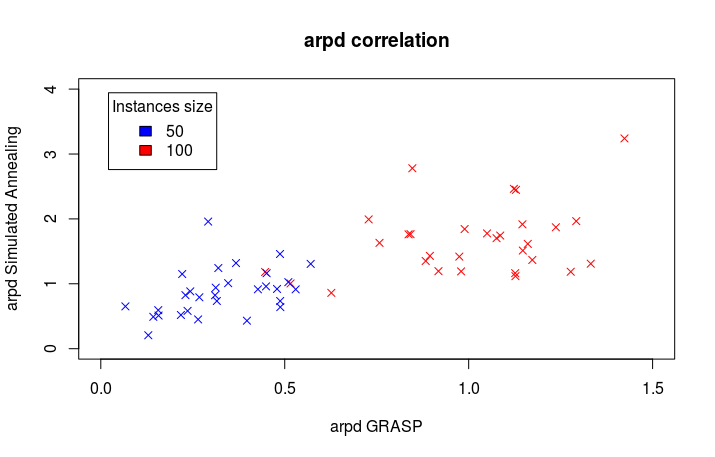
\includegraphics[scale=0.5]{images/correlation}
    \caption{Correlation plot between the arpd's}
    \label{fig:corr}
\end{figure}

The figure \ref{fig:corr} shows the correlation between the average relative percentage deviations of the solutions of all instances returned by the two algorithms.
The blue crosses correspond to the instances of size $50$ and the red crosses correspond to the instances of size $100$.

We can see that there is a difference between the instances of size $50$ and the instances of size $100$.
It seems that there is a correlation for instances of size $50$.
However, for instances of size $100$, no correlation is visible.\newline

A statistical test can be used to confirm the results again.
A spearman test with a significance level equal to $0.05$ gives a p-value equal to $0.003$ for instances of size $50$ and a p-value equal to 0$.21$ for instances of size $100$.
This results confirm the previous discussion, as the null hypothesis is rejected for instances of size $50$.\newline

These results show that the SA algorithm may be improved to obtain better qualities on the easiest instances (according to the arpd's of GRASP).
The warming step introduced may be inefficient and a bigger neighbourhood like the insert one could be better for this algorithm.

\subsection{Run-time distributions}

The figures \ref{fig:rt_sa} and \ref{fig:rt_grasp} show the Qualified run time distributions of the algorithms.
This plots are obtained with 25 runs of the algorithms on the first 5 instances of size 50 with a time limit equal to ten times the previous one (for size 50).
As the algorithms do not necessarily reach the best known solutions, the run time distribution has been computed for $0.1$, $0.2$ and $1.2$ percents of the best known solution.
The tests have been performed on Ubuntu 16.04 with a Intel Core i3-3110M CPU 2.40GHz. \newline

We can observe on the plots of the two algorithms that the probabilty of reaching 1.2\% of the best solution is quite high from the beginning of the algorithm.
However, the probability ton reach 0.1\% remains low at the begining of the runs.

On the both plots, the black curve corresponds to an exponential distribution.
On the GRASP plot, the distribution is $1-2^{-\frac{x}{17}}$ and on the SA plot, the distribution is $1-2^{-\frac{x}{100}}$.
On the grasp plot, wa can see that the exponential distribution does not fit completely with the qualified run time distribution, which means that the algorithm can be slightly improved with restarts.\newline

The figure \ref{fig:rt_comp} shows the comparison between the qualified run time distribution for both algorithms with a goal equal to $0.5\%$ of the best known solution.
We can observe that the GRASP run time distribution dominates the SA one.
Indeed, all the time, the probability to reach the goal is higher with GRASP.
It confirms the hypothesis that this implementation of GRASP is better than the one of Simulated Annealing.

\begin{figure}
    \centering
        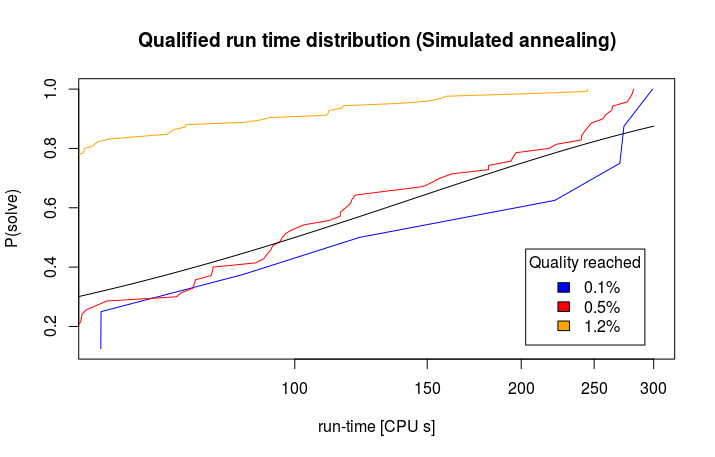
\includegraphics[scale=0.5]{images/rt_sa}
    \caption{Qualified run time distribution of simulated annealing}
    \label{fig:rt_sa}
\end{figure}

\begin{figure}
    \centering
        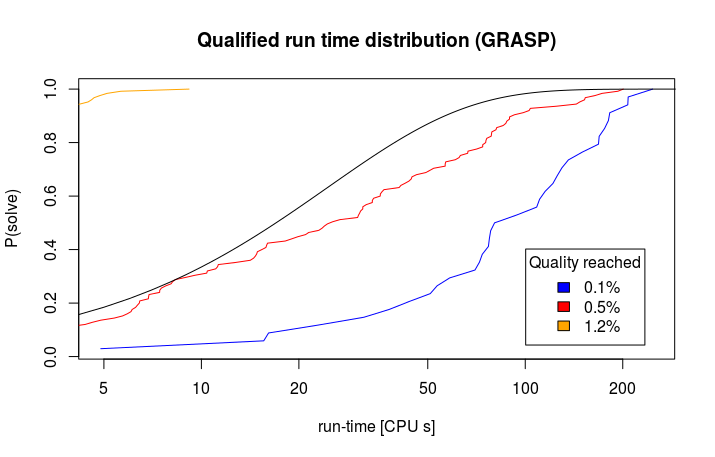
\includegraphics[scale=0.5]{images/rt_grasp}
    \caption{Qualified run time distribution of GRASP}
    \label{fig:rt_grasp}
\end{figure}

\begin{figure}
    \centering
        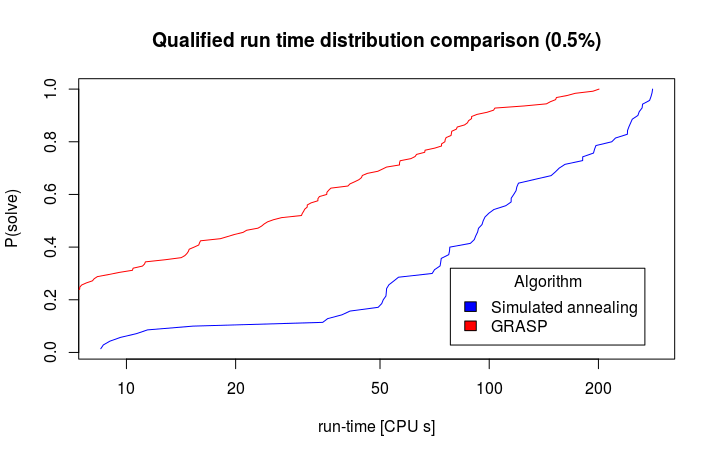
\includegraphics[scale=0.5]{images/rt_comp}
    \caption{Comparison of qualified run time distributions}
    \label{fig:rt_comp}
\end{figure}


\section{Conclusion}

To conclude, the results show that the GRASP implementation is better than the SA one.
The means, the statistical tests and the comparison of the qualified run time distributions give strong evidences.\newline

However, the behaviour of the Simulated annealing is odd.
The correlation plot shows that all the instances of size 100 seem to have the same difficulty with this algorithm.
It is possible that bad choices were made during the implementation.
A possible explanation is the use of the transpose neighbourhood (it was done to keep a small neighbourhood, in order to keep a low number of iterations for each temperature value).
To improve the result, it should be interesting to test with the insert neighbourhood.
The warming step could also be inefficient in this case.\newline

To finish, it seems that GRASP can still be improved, as shown by the qualified run time distribution.

% \section{better solution found}
% 50\_20\_03 \newline
% 1 28 24 14 48 15 34 45 19 5 18 37 11 29 31 9 39 10 25 33 30 44 2 43 7 41 20 40 49 47 38 4 42 17 16 22 6 26 8 50 13 21 32 23 46 36 35 3 12 27 \newline
% 591806

\begin{thebibliography}{12}

\bibitem{ref} Q.-K. Pan, R. Ruiz.
2012.
Local search methods for the flowshop scheduling problem with flowtime minimization.
European Journal of Operational Research 222(1), 31-43.

\end{thebibliography}

\end{document}
